\documentclass[a4paper,14pt]{extarticle}
% Thay doi chieu cao cua header va top margin
% de fix warning `\headheight is too small`
\setlength{\headheight}{17pt}
\addtolength{\topmargin}{-3pt}

% Package render ngon ngu tieng Viet
\usepackage[utf8]{vietnam}

% Package can le tren, duoi, trai, phai
\usepackage[left=3.5cm,right=2.5cm,top=3cm,bottom=3cm]{geometry}

% Packages de viet cong thuc Toan hoc
\usepackage{amsmath,amssymb, amsthm}
% Package de viet in dam cong thuc Toan hoc (bm = bold math)
\usepackage{bm}

% Package su dung de giu figure/table o dung vi tri
% \begin{figure}[H]
%     ... figure contents...
% \end{figure}
% Note: can check lai (comment ko thay khac biet)
\usepackage{float}

% Package custom style cua caption
% (kich thuoc font chu, khoang cach so voi anh, ...)
\usepackage[font=small,skip=0pt]{caption}

% Package custom khoang cach
% giua cac gach dau dong trong danh sach
\usepackage{enumitem}
\setlist{nosep}

% Custom khoang cach giua cac dong (gian dong)
% Note: can check lai dong `usepackage` (comment ko thay khac biet)
\usepackage{setspace}
\renewcommand{\baselinestretch}{1.25}

% Package su dung font Times la font cho text va
% cung cap mot so syntax Toan hoc
\usepackage{mathptmx}

% Package su dung de reference/citation co the click
\usepackage{hyperref}

% Package su dung cho viec danh `chi muc tu khoa`
\usepackage{imakeidx}
\makeindex[columns=2, columnsep=0.5em, title=Chỉ mục từ khoá, intoc]

% Package su dung cho `khungtrangbia`
\usepackage{tikz}

% Package su dung cho `pythoncodestyle`
\usepackage{listings}

% Package su dung cho `headerfooterstyle`
\usepackage{fancyhdr}

% Custom style cho header and footer
% De su dung duoc custom style nay, can `\usepackage{fancyhdr}`
\def\headerfooterstyle{
    \pagestyle{fancy}
    \fancyhf{}
    \lhead{\thesection}
    \rhead{\thepage}
    \lfoot{}
    \rfoot{Nguyễn Hữu Minh}
    \renewcommand{\headrulewidth}{2pt}
    \renewcommand{\footrulewidth}{1pt}
}

\headerfooterstyle

% Package su dung de ve bang `tab_result` trong file `4_munit_results.tex`
\usepackage[flushleft]{threeparttable}

% Khai bao ky tu unicode de sua error
% Package inputenc: Unicode character − (U+2212) (inputenc) not set up for use with LaTeX.
\DeclareUnicodeCharacter{2212}{-}

\begin{document}

    % BAT DAU CAC TRANG CHUC NANG
    % Xoa page number
    \pagenumbering{gobble}
    % Xoa header - footer
    \pagestyle{plain}

    
\def\trangbia{
    % % De dung "khung_trang_bia", ta can `\usepackage{tikz}`
    % 
% De su dung "khungtrangbia", ta can `\usepackage{tikz}`
\def\khungtrangbia{
  \begin{tikzpicture}[remember picture,overlay,inner sep=0,outer sep=0]
    \draw[black!70!black,line width=3pt]([xshift=-2cm,yshift=-2.5cm]current page.north east)
    coordinate (A) -- ([xshift=2.5cm,yshift=-2.5cm]current page.north west)
    coordinate (B) -- ([xshift=2.5cm,yshift=2.5cm]current page.south west)
    coordinate (C) -- ([xshift=-2cm,yshift=2.5cm]current page.south east)
    coordinate (D) -- cycle;
    \draw ([yshift=0.5cm,xshift=-0.5cm]A) --
    ([yshift=0.5cm,xshift=0.5cm]B) --
    ([yshift=-0.5cm,xshift=0.5cm]B) --
    ([yshift=-0.5cm,xshift=-0.5cm]B) --
    ([yshift=0.5cm,xshift=-0.5cm]C) --
    ([yshift=0.5cm,xshift=0.5cm]C) --
    ([yshift=-0.5cm,xshift=0.5cm]C) --
    ([yshift=-0.5cm,xshift=-0.5cm]D) --
    ([yshift=0.5cm,xshift=-0.5cm]D) --
    ([yshift=0.5cm,xshift=0.5cm]D) --
    ([yshift=-0.5cm,xshift=0.5cm]A) --
    ([yshift=-0.5cm,xshift=-0.5cm]A) --
    ([yshift=0.5cm,xshift=-0.5cm]A);
    \draw ([yshift=-0.3cm,xshift=0.3cm]A) --
    ([yshift=-0.3cm,xshift=-0.3cm]B) --
    ([yshift=0.3cm,xshift=-0.3cm]B) --
    ([yshift=0.3cm,xshift=0.3cm]B) --
    ([yshift=-0.3cm,xshift=0.3cm]C) --
    ([yshift=-0.3cm,xshift=-0.3cm]C) --
    ([yshift=0.3cm,xshift=-0.3cm]C) --
    ([yshift=0.3cm,xshift=0.3cm]D) --
    ([yshift=-0.3cm,xshift=0.3cm]D) --
    ([yshift=-0.3cm,xshift=-0.3cm]D) --
    ([yshift=0.3cm,xshift=-0.3cm]A) --
    ([yshift=0.3cm,xshift=0.3cm]A) --
    ([yshift=-0.3cm,xshift=0.3cm]A);
  \end{tikzpicture}
}

    % \vekhungtrangbia
    
    \large {\bf \centerline {TRƯỜNG ĐẠI HỌC BÁCH KHOA HÀ NỘI}}
    \vskip 0.6in

    % \begin{center}
    %     
\includegraphics[width=0.25\columnwidth]{images/logo_bk.png}
    % \end{center}
    \vskip 0.5in

    \LARGE {\bf \centerline {LUẬN VĂN THẠC SĨ}}
    \vskip 0.6in

    \LARGE {\bf \centerline {Ứng dụng mô hình học sâu}}
    \LARGE {\bf \centerline {giải quyết một số bài toán}}
    \LARGE {\bf \centerline {phân tích và xử lý hình ảnh}}
    \vskip 0.6in

    \hspace{3cm}
    \normalsize {\bf NGUYỄN HỮU MINH}
    \vskip 0in
    \hspace{3cm}
    \normalsize {}
    \vskip 0in
    \hspace{3cm}
    \normalsize {\textbf{Ngành}: Toán Tin}
    \vskip 0in
    \hspace{3cm}
    \normalsize {\textbf{Chuyên ngành}: Toán Tin}
    \vskip 1.3in

    \hspace{0.5cm}
    \small {\textbf{Giảng viên hướng dẫn}: ......................................}
    \hspace{0.5cm}
    \begin{tikzpicture}
        \draw (15.5,0)--(18.5,0);
    \end{tikzpicture}
    \vskip 0in

    \hspace{0.5cm}
    \small {\textbf{Bộ môn}: Toán Tin \hspace{5.7cm} Chữ ký của GVHD}
    \vskip 0in

    \hspace{0.5cm}
    \small {\textbf{Viện}: Toán ứng dụng và Tin học}
    \vskip 1.2in
  
    \small {\centerline {Hà Nội, 06/2020}}
}

    \trangbia

    \newpage
    
\def\nhanxet{
    \large {\bf {\centerline {NHẬN XÉT CỦA GIẢNG VIÊN HƯỚNG DẪN}}}
    \vskip 0.5in

    \normalsize {\bf \flushleft{1. Mục đích và nội dung của đồ án:}}
    \vskip 2in

    \normalsize {\bf \flushleft{2. Kết quả đạt được:}}
    \vskip 2in

    \normalsize {\bf \flushleft{3. Ý thức làm việc của sinh viên:}}
    \vskip 2in

    \hspace{8cm}
    \normalsize {Hà Nội, ngày \hspace{0.5cm} tháng \hspace{0.5cm} năm}
    \vskip 0in

    \hspace{8.5cm}
    \normalsize {\textit{Giảng viên hướng dẫn}}
}

    \nhanxet

    \newpage
    
\def\loicamon{
    \section*{Lời cảm ơn}
    \addcontentsline{toc}{section}{Lời cảm ơn}
    Với tấm lòng biết ơn vô cùng sâu sắc, tôi xin gửi lời cảm ơn chân thành nhất đến quý Thầy Cô của Viện Toán ứng dụng và Tin học, Đại học Bách Khoa Hà Nội đã tạo điều kiện và dành cho tôi vốn kiến thức quý báu. \\
    Đặc biệt, tôi xin chân thành cảm ơn ThS. --------- đã tận tâm hướng dẫn tôi trong suốt thời gian vừa qua.
    Nhờ có những lời hướng dẫn của thầy mà luận văn của tôi đã hoàn thành một cách tốt nhất. \\
    Tôi rất mong nhận được ý kiến đóng góp của quý Thầy Cô và các bạn học để luận văn của ôi được hoàn thiện hơn.
    Tôi xin chân thành cảm ơn!
}

    \loicamon

    % Bat dau danh so trang page number
    \pagenumbering{arabic}

    \newpage
    
\def \tomtatnoidung{
    \section*{Tóm tắt nội dung đồ án}
    \addcontentsline{toc}{section}{Tóm tắt nội dung đồ án}
    Cách mạng công nghiệp 4.0 đã mang đến cho con người một kỷ nguyên khai phá dữ liệu. Điều này đặt ra bài toán không chỉ làm sao để khai phá được dữ liệu một cách hiệu quả mà còn làm sao để sinh ra được thêm nhiều dữ liệu một cách tự động và với số lượng lớn. Do đó, trong khuôn khổ của đồ án tốt nghiệp, em sẽ nghiên cứu về ý tưởng chung, kiến trúc, hàm loss, phương pháp đánh giá, những vấn đề tồn đọng và cách giải quyết các vấn đề đó của mô hình Generative Adversarial Networks (GANs) tổng quát nhằm giải quyết bài toán sinh dữ liệu ảnh nói và mô hình Multimodal Unsupervised Image-to-Image Translation (MUNIT) giúp giải quyết bài toán sinh dữ liệu ảnh mới từ ảnh đã có sẵn (Image-to-Image Translation). Bên cạnh những kết quả đã được công bố trong bài báo, em đã thử nghiệm mô hình với bộ dữ liệu khác để chứng minh tính đúng đắn của mô hình và lấy đó làm tiền đề cho việc phát triển những mô hình phức tạp hơn trong tương lai.
    \vskip 2.5in

    \hspace{7.7cm}
    \normalsize {Hà Nội, ngày \hspace{0.5cm} tháng \hspace{0.5cm} năm}
    \vskip 0in

    \hspace{8.5cm}
    \normalsize {\textit{Sinh viên thực hiện}}
}
    \tomtatnoidung

    \newpage
    \tableofcontents

    \newpage
    \listoffigures
    \addcontentsline{toc}{section}{Danh sách hình vẽ}

    \newpage
    \listoftables
    \addcontentsline{toc}{section}{Danh sách bảng}
    % KET THUC CAC TRANG CHUC NANG

    % BAT DAU PHAN NOI DUNG CHINH
    % Bat dau hien header - footer tu trang nay ve sau
    \pagestyle{fancy}

    \newpage
    hello content \cite{test}


    \newpage


    \newpage


    \newpage

    % % KET THUC PHAN NOI DUNG CHINH

    % BAT DAU CAC TRANG CHUC NANG KHAC
    % Xoa header - footer
    \pagestyle{plain}

    \newpage
    \def \tongket{
    \section*{Kết luận và phương hướng phát triển}
    \addcontentsline{toc}{section}{Kết luận và phương hướng phát triển}
    Với sự phát triển của khoa học công nghệ, kích thước của ảnh trong thực tế cuộc sống ngày càng tăng và điều đó đòi hỏi các mô hình học sâu xử lý với độ chính xác cao và tốc độ nhanh.
    Rào cản này đã phần nào đó được vượt qua thông qua các nghiên cứu trong những năm trở lại đây, giúp việc xử lý ảnh chất lượng cao trở nên dễ dàng và chính xác hơn. \\
    Hai đóng góp chính của luận văn bao gồm: \\
    - Mô hình RetinaFocus giúp cải thiện độ chính xác và tốc độ của các mô hình học sâu giải quyết bài toán nhận diện khuôn mặt với trong ảnh chất lượng cao rất nhiều.
    So sánh với mô hình nguyên bản, mô hình RetinaFocus đã tăng tốc ... trong khi duy trì được độ chính xác tương đương trên bộ dữ liệu WIDER FACE. \\
    - Bộ dữ liệu WIDER FACE kích thước lớn đã giúp đánh giá một cách chính xác và khách quan độ chính xác và tốc độ của mô hình RetinaFocus trong việc xử lý ảnh chất lượng cao, so sánh với kết quả của mô hình nguyên bản. \\
    Từ đó, mô hình RetinaFocus sẽ là nền tảng cho các nghiên cứu khác giải quyết bài toán nhận diện khuôn mặt cũng như là nhận diện đối tượng\index{nhận diện đối tượng} trong ảnh chất lượng cao trong tương lai.
}
    \tongket

    \newpage
    \printindex


    \newpage
    \def \code{
    % De su dung "pythoncodestyle", ta can `\usepackage{listings}`
    
% De su dung "pythoncodestyle", ta can `\usepackage{listings}`
\def\pythoncodestyle{
    % color and style for code
    \definecolor{codegreen}{rgb}{0,0.6,0}
    \definecolor{codegray}{rgb}{0.5,0.5,0.5}
    \definecolor{codepurple}{rgb}{0.58,0,0.82}
    \definecolor{backcolour}{rgb}{0.95,0.95,0.92}
    \lstdefinestyle{mycodingstyle}{
        backgroundcolor=\color{backcolour},   
        commentstyle=\color{codegreen},
        keywordstyle=\color{magenta},
        numberstyle=\tiny\color{codegray},
        stringstyle=\color{codepurple},
        basicstyle=\ttfamily\footnotesize,
        breakatwhitespace=false,         
        breaklines=true,                 
        captionpos=b,                    
        keepspaces=true,                 
        numbers=left,                    
        numbersep=5pt,                  
        showspaces=false,                
        showstringspaces=false,
        showtabs=false,                  
        tabsize=2
    }
    \lstset{style=mycodingstyle}
}
    \pythoncodestyle

    \section*{Phụ lục}
    \addcontentsline{toc}{section}{Phụ lục}
    \subsection*{Phụ lục 1: Một số đoạn code}
    \subsubsection*{Lập trình Content Encoder}
    \lstinputlisting[language=Python]{codes/content_encoder.py}
    \subsubsection*{Lập trình Style Encoder}
    \lstinputlisting[language=Python]{codes/style_encoder.py}
    \subsubsection*{Lập trình Decoder}
    \lstinputlisting[language=Python]{codes/decoder.py}
    \subsubsection*{Lập trình Generator}
    \lstinputlisting[language=Python]{codes/generator.py}
    \subsubsection*{Lập trình Discriminator}
    \lstinputlisting[language=Python]{codes/discriminator.py}
    \subsubsection*{Lập trình các hàm loss}
    \lstinputlisting[language=Python]{codes/loss.py}
}
    \code

    \newpage
    \addcontentsline{toc}{section}{Tài liệu tham khảo}
    \renewcommand\refname{Tài liệu tham khảo}
    \bibliography{references.bib}
    \bibliographystyle{unsrt}
    % KET THUC CAC TRANG CHUC NANG KHAC

\end{document}